\chapter{Przebieg badań}
\fancyhead[C]{PRZEBIEG BADAŃ}
\fancyhead[L]{}
\fancyhead[R]{}

\section{Obrane założenia}
\begin{enumerate}
	\item Przez wzgląd na duży rozmiar wygenerowanych grafów wybranych do wykonania projektu, w celu przeprowadzenia obliczeń wykorzystano\textbf{ MacBook Pro z procesorem  Intel Core i7-6820HQ oraz 16 GB pamięci RAM}.
	\item Minimalna liczba iteracji, wystarczająca do wykonania badań, to \textbf{100}, jednak przez wzgląd na możliwości sprzętowe, zdecydowano się na liczbę iteracji równą \textbf{1000}.
	\item Badania przeprowadzono dla grafów o \textbf{liczbie wierzchołków} równej: 10, 50, 100, 500, 1000, 5000 oraz 10 000.
	\item Badania przeprowadzono dla grafów o \textbf{gęstości} równej: 0.2, 0.4, 0.6, 0.8 oraz 1.0.
\end{enumerate}

\newpage
\section{Przebieg obliczeń}
Aby określić liczbę iteracji, przeprowadzono testy na grafie pełnym o 1000 wierzchołkach. Wyniki tych badań prezentuje tabela \ref{fig: tab1}.

\begin{figure}[htb!]
	\centering
	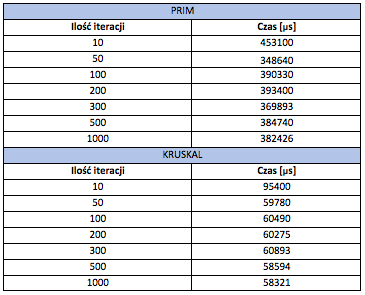
\includegraphics[width=0.5\textwidth]{tex/fig/tab1}
	\caption{Wyniki badań czasu wykonania algorytmów dla różnej liczby iteracji.}
	\label{fig: tab1}
\end{figure}
%%%%%%%%%%%%%%%%%%%%%%%%%%%%%%%%%%%%%%%%%%%%%%%%%%%%%%%%%%%%%%%%%%%%%%%%%%%%%%%%%%%%%%%%%%%%%%%%%%%%%%%%%%%%%%%%%%%%%%%%

Z tabeli \ref{fig: tab1} wynika, że minimalną liczbą iteracji dla prowadzonych obliczeń jest liczba 100, ponieważ  wartości czasu wykonania algorytmu dla większych od niej liczb iteracji niewiele się od siebie różnią. \textbf{Jednak dzięki dostępnym możliwościom sprzętowym zdecydowano się na ustawienie liczby iteracji równej 1000.}
%%%%%%%%%%%%%%%%%%%%%%%%%%%%%%%%%%%%%%%%%%%%%%%%%%%%%%%%%%%%%%%%%%%%%%%%%%%%%%%%%%%%%%%%%%%%%%%%%%%%%%%%%%%%%%%%%%%%%%%%
\newpage
Następnie obliczono liczbę krawędzi dla grafów o danej liczbie wierzchołków oraz zakładanej gęstości. Wyniki obliczeń, zarazem zbiór danych grafów wejściowych, prezentuje tabela \ref{fig: tab2}.

\begin{figure}[htb!]
	\centering
	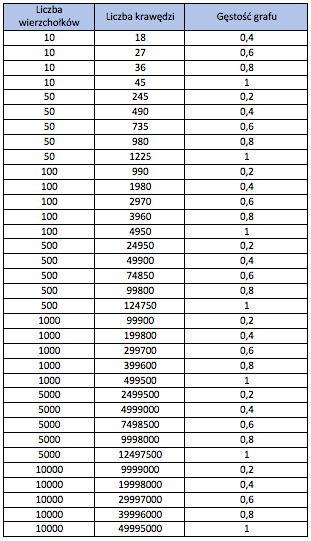
\includegraphics[width=0.5\textwidth]{tex/fig/tab2}
	\caption{Dane niezbędne do wygenerowania grafu o określonych parametrach.}
	\label{fig: tab2}
\end{figure}

\newpage 
Po ustawieniu liczby iteracji w programie, przystąpiono do wykonania obliczeń w następujący sposób:
\begin{enumerate}
	\item Wygenerowano graf o zadanych parametrach.
	\item Po wygenerowaniu grafu uruchomiono algorytm Prima.
	\item Po wykonaniu wszystkich iteracji dla algorytmu Prima, uruchomiono algorytm Kruskala.
\end{enumerate}


\subsection{Weryfikacja poprawności implementacji algorytmów}
Algorytmy zostały przetestowane na grafach dla których znane jest poprawne MST. Następnie porównane zostały wyniki obu algorytmów dla pewnych grafów losowych. 
Podczas wszystkich przeprowadzonych testów liczone i porównywane były nie tylko zbiory krawędzi tworzących MST, ale również sumy wag tych krawędzi.

Wstępne obliczenia dla grafu pełnego o 1000 wierzchołkach wykazały dużą rozbieżność pomiędzy wynikami czasu wykonania dla obu algorytmów (na niekorzyść Prima). 
Wpływ na zaistniałą sytuację miały następujące czynniki:
\begin{enumerate}
	\item Niewłaściwy sposób pomiaru czasu dla algorytmu Kruskala - pominięto sortowanie  krawędzi na początku algorytmu.
	\item Struktura reprezentująca graf -- algorytm Prima zoptymalizowano dzięki wykorzystaniu do tego celu list sąsiedztwa (zamiast macierzy sąsiedztwa).
\end{enumerate}

Wyniki przeprowadzonych obliczeń zaprezentowano w sekcji \ref{results}.
\newpage
\section{Wyniki eksperymentu}
\label{results}
Po dokonaniu optymalizacji i poprawy zaistniałych niedociągnięć wykonano obliczenia, których wyniki zestawiono w tabeli \ref{fig: tab3}.
\begin{figure}[htb!]
	\centering
	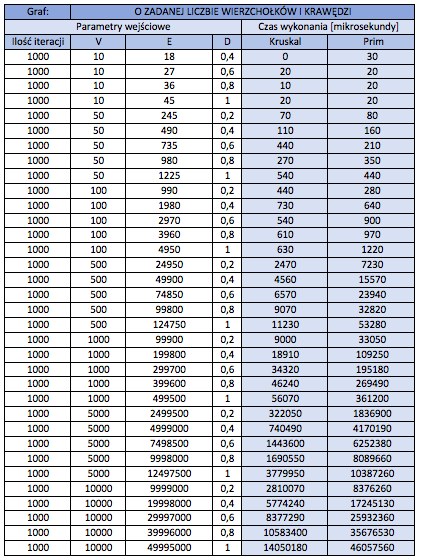
\includegraphics[width=0.8\textwidth]{tex/fig/tab3}
	\caption{Wyniki obliczeń dla obu algorytmów.}
	\label{fig: tab3}
\end{figure}

\newpage
Otrzymane wyniki przedstawiono również w formie wykresów:
\begin{itemize}
 \item Zależność czasu wykonania algorytmu Prima od gęstości D danych grafów prezentuje wykres \ref{fig: w1}. 
 
 \begin{figure}[htb!]
 	\centering
 	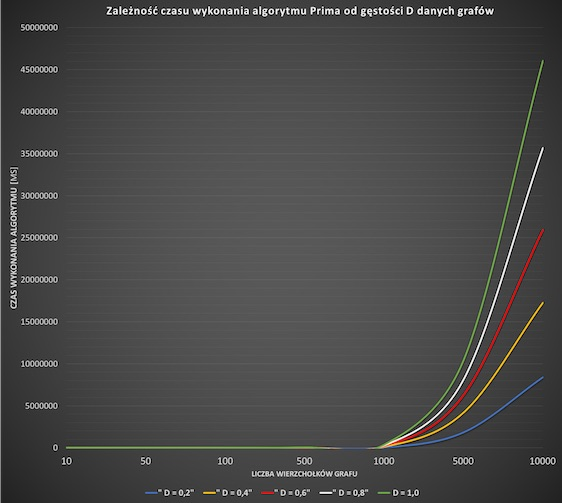
\includegraphics[width=1 \textwidth]{tex/fig/p1}
 	\caption{Zależność czasu wykonania algorytmu Prima od gęstości D danych grafów.}
 	\label{fig: w1}
 \end{figure}

\newpage
 Wykres ten został też podzielony na dwie części w celu zwiększenia czytelności:
 \begin{enumerate}
 	\item Zależność czasu wykonania algorytmu Prima od gęstości grafów o liczbie wierzchołków V$\subseteq$\{10,50,100,500,1000\} - rys. \ref{fig: ww1}
 	
 	 \begin{figure}[htb!]
 		\centering
 		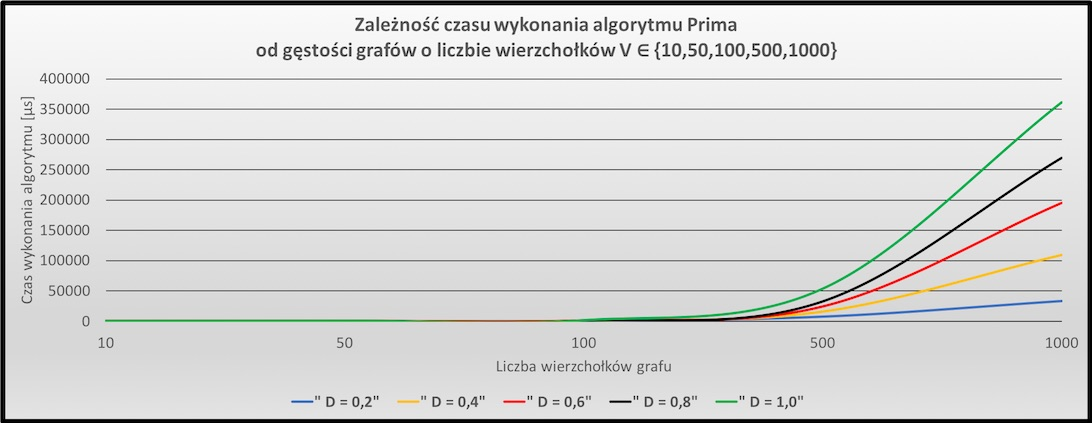
\includegraphics[width=1\textwidth]{tex/fig/p2_10_1000}
 		\caption{Zależność czasu wykonania algorytmu Prima od gęstości grafów o liczbie wierzchołków V$\subseteq$ \{10,50,100,500,1000\}}
 		\label{fig: ww1}
 	\end{figure}
 
 	\item Zależność czasu wykonania algorytmu Prima od gęstości grafów o liczbie wierzchołków V$\subseteq$ \{500,1000,5000,10000\} - rys. \ref{fig: ww11}.
 	
 	 \begin{figure}[htb!]
 		\centering
 		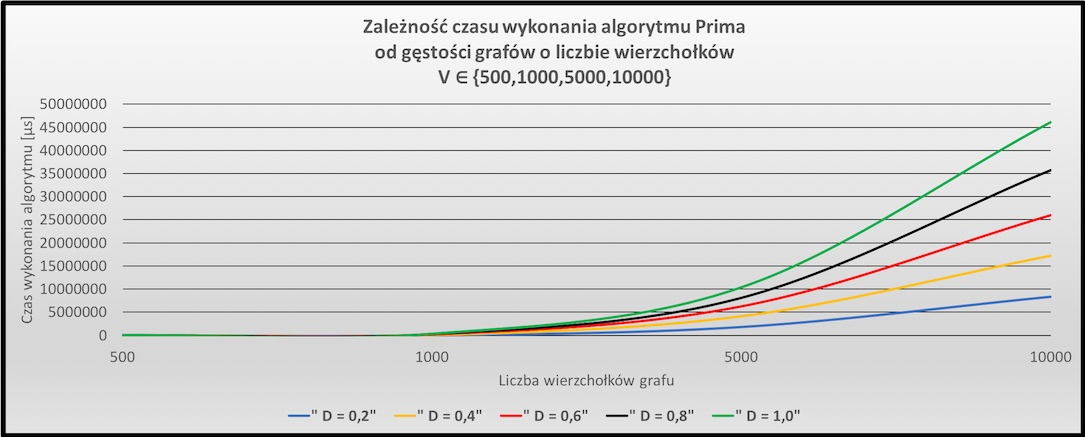
\includegraphics[width=1\textwidth]{tex/fig/p22}
 		\caption{Zależność czasu wykonania algorytmu Prima od gęstości grafów o liczbie wierzchołków V$\subseteq$ \{500,1000,5000,10000\} } 
 		\label{fig: ww11}
 	\end{figure}
 
 \end{enumerate}
\newpage
 \item Zależność czasu wykonania algorytmu Kruskala od gęstości D danych grafów prezentuje wykres \ref{fig: w2}. 
 
  \begin{figure}[htb!]
 	\centering
 	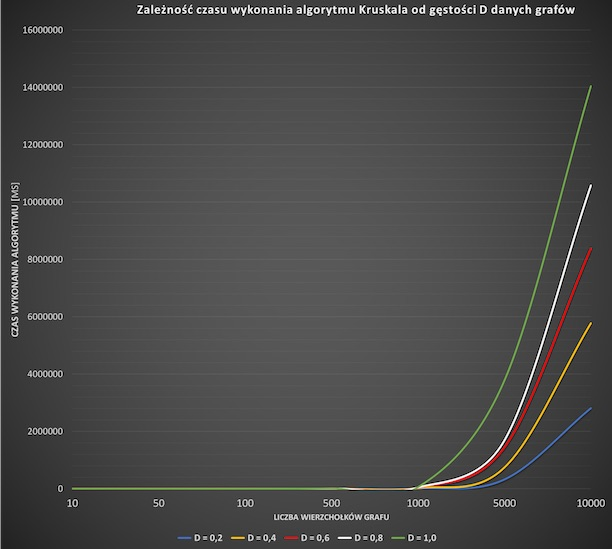
\includegraphics[width=1\textwidth]{tex/fig/k1}
 	\caption{Zależność czasu wykonania algorytmu Kruskala od gęstości D danych grafów.}
 	\label{fig: w2}
 \end{figure}

\newpage
 Wykres ten został też podzielony na dwie części w celu zwiększenia czytelności:
  \begin{enumerate}
 	\item Zależność czasu wykonania algorytmu Kruskala od gęstości grafów o liczbie wierzchołków V$\subseteq$ \{10,50,100,500,1000\}- rys. \ref{fig: ww2}
 	
\begin{figure}[htb!]
	\centering
	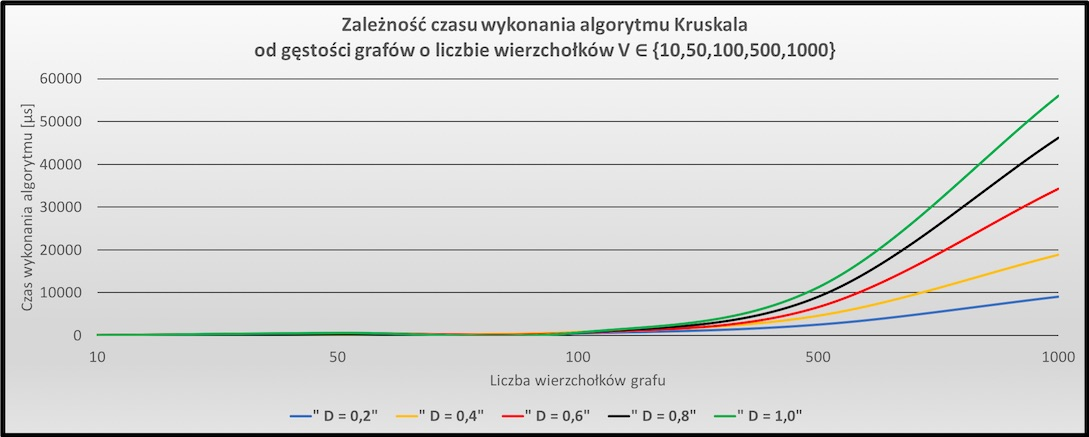
\includegraphics[width=1\textwidth]{tex/fig/k2_10_1000}
	\caption{Zależność czasu wykonania algorytmu Kruskala od gęstości grafów o liczbie wierzchołków V$\subseteq$ \{10,50,100,500,1000\}}
	\label{fig: ww2}
\end{figure}

 	\item Zależność czasu wykonania algorytmu Kruskala od gęstości grafów o liczbie wierzchołków V$\subseteq$ \{500,1000,5000,10000\}  - rys. \ref{fig: ww2}.
 	
 	\begin{figure}[htb!]
 		\centering
 		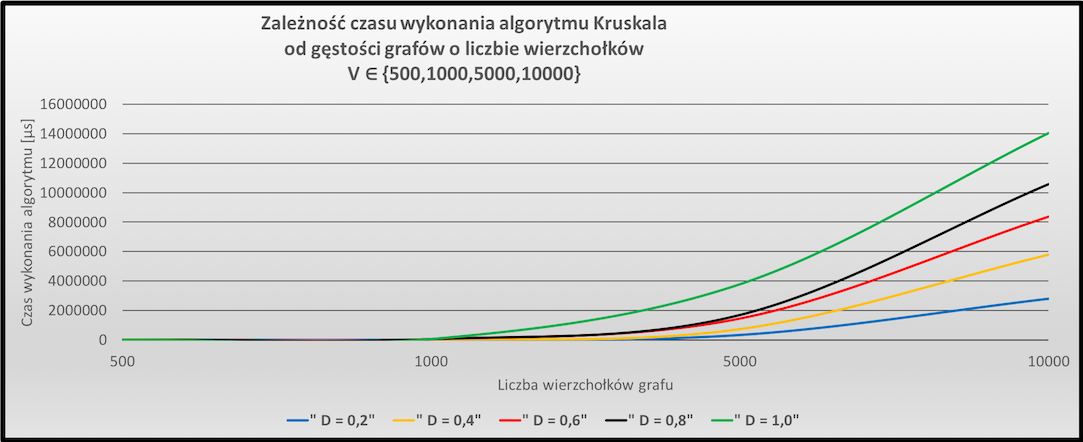
\includegraphics[width=1\textwidth]{tex/fig/k22}
 		\caption{Zależność czasu wykonania algorytmu Kruskala od gęstości grafów o liczbie wierzchołków V$\subseteq$ \{500,1000,5000,10000\} }
 		\label{fig: ww22}
 	\end{figure}
 \end{enumerate}

\item Zestawienie czasów wykonania algorytmów Prima i Kruskala dla grafów o zadanych parametrach z kolei prezentuje rys. \ref{fig: pk1}.
	\begin{figure}[htb!]
	\centering
	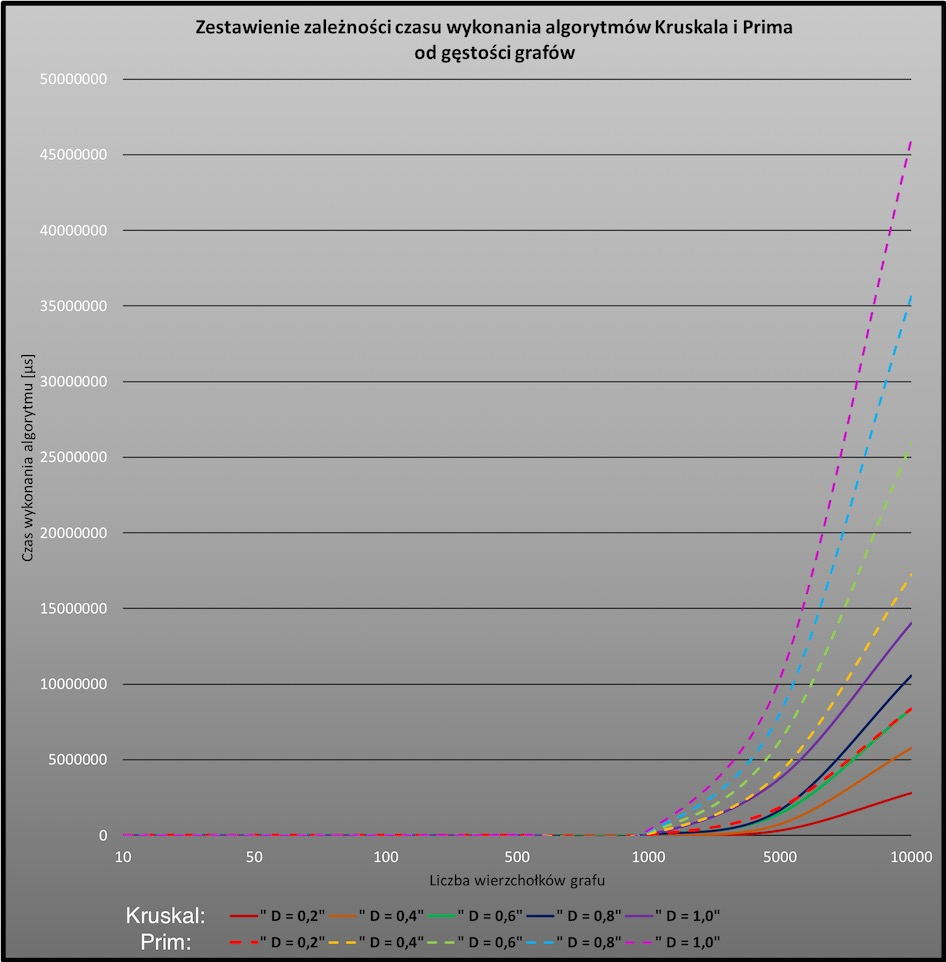
\includegraphics[width=1\textwidth]{tex/fig/kp1}
	\caption{Zestawienie zależności czasów wykonania algorytmów Prima i Kruskala od gęstości grafów}
	\label{fig: pk1}
\end{figure}
\newpage
Diagram ten jest podstawą dla wniosków wysuniętych w sekcji \ref{conclusion}. Dla poprawy czytelności podzielono go na dwie części:
\begin{enumerate}
	\item Zestawienie zależności czasu wykonania algorytmów Kruskala i Prima od gęstości grafów o liczbie wierzchołków V$\subseteq$ \{10,50,100,500,1000\} - rys. \ref{fig: kp1}.
	
		\begin{figure}[htb!]
		\centering
		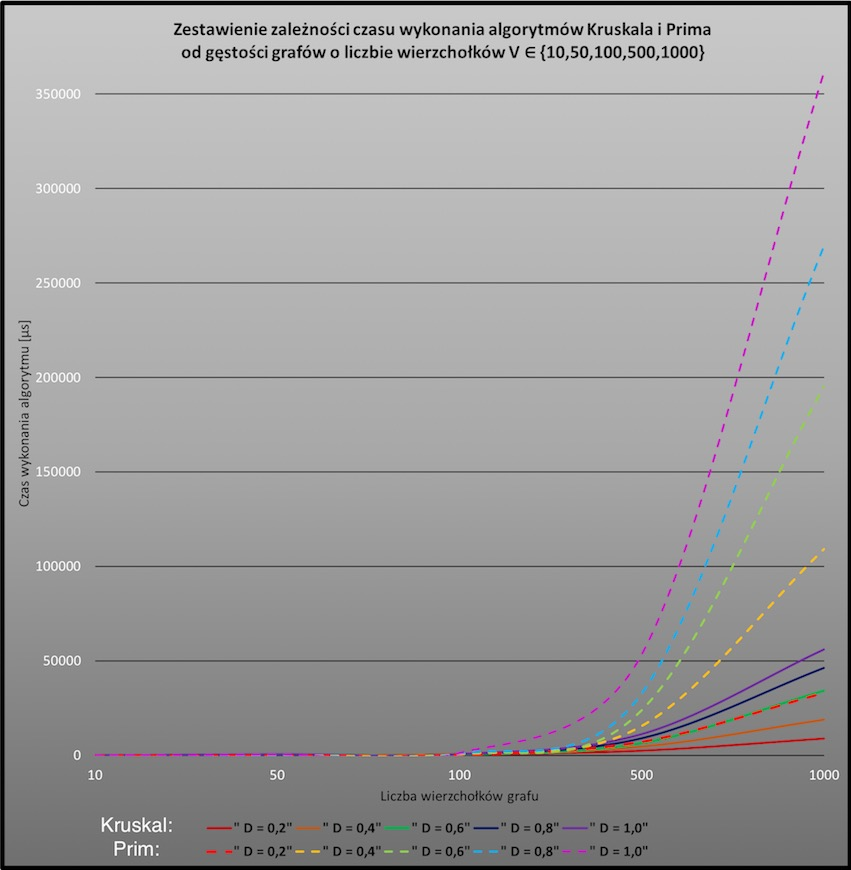
\includegraphics[width=1\textwidth]{tex/fig/kp_10_1000}
		\caption{Zestawienie zależności czasu wykonania algorytmów Kruskala i Prima od gęstości grafów o liczbie wierzchołków V$\subseteq$ \{10,50,100,500,1000\}}
		\label{fig: kp1}
	\end{figure}

\item Zestawienie zależności czasu wykonania algorytmów Kruskala i Prima od gęstości grafów o liczbie wierzchołków V$\subseteq$ \{500,1000,5000,10000\}  - rys. \ref{fig: kp2}.
\begin{figure}[htb!]
	\centering
	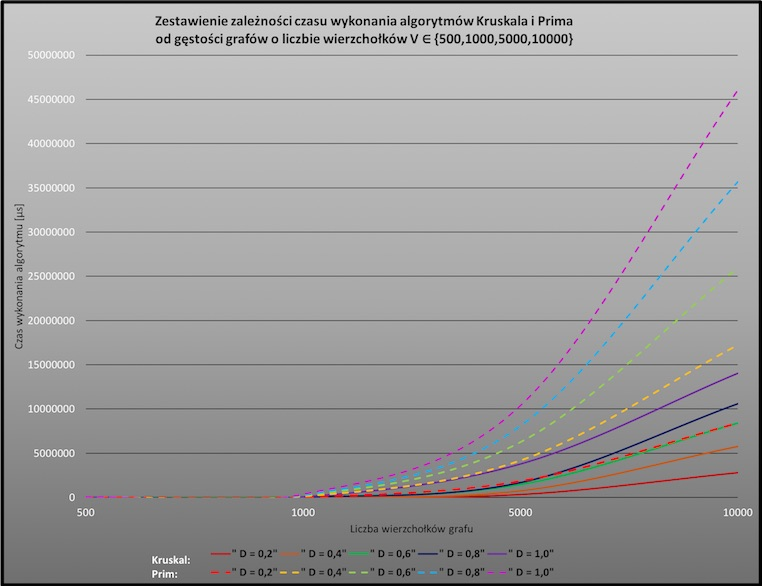
\includegraphics[width=1\textwidth]{tex/fig/kp_500_1000}
	\caption{Zestawienie zależności czasu wykonania algorytmów Kruskala i Prima od gęstości grafów o liczbie wierzchołków V$\subseteq$ \{500,1000,5000,10000\} }
	\label{fig: kp2}
\end{figure}
\end{enumerate}
\end{itemize}

\newpage
\section{Wnioski}
\fancyhead[C]{WNIOSKI}
\fancyhead[L]{}
\fancyhead[R]{}
\label{conclusion}
Na podstawie powyższych wyników obliczeń wyciągnięto następujące wnioski:
\begin{enumerate}
	\item Dla małych grafów algorytm Prima uzyskuje porównywalne (a nawet lepsze) wyniki względem algorytmu Kruskala
	\item W przypadku dużych grafów zastosowanie algorytmu Kruskala sprawdza się lepiej przez wzgląd na krótszy czas wykonywania 
	\item Z diagramu wynika, że algorytm Prima ma dłuższy czas wykonywania od algorytmu Kruskala
	\item W przypadku grafów o małej gęstości algorytm Kruskala radzi sobie znacznie lepiej od algorytmu Prima
	\item Różnice czasu wykonywania algorytmu wynikają z:\\
	-- Implementacji każdego z algorytmów\\
	-- Wykorzystanych do implementacji struktur danych\\
	-- Doboru odpowiednich parametrów generowanego do obliczeń grafu
\end{enumerate}


